\documentclass{article}
\usepackage{graphicx}
\usepackage{amssymb}
\usepackage{amsmath}
\usepackage{tikz}
\usepackage{url}
\usepackage{color}
\usetikzlibrary{shapes}


\linespread{1.4}
\setlength{\parindent}{0pt}
\setlength{\parskip}{1.9ex plus 0.5ex minus 0.2ex}

\title{Hop, Jump and Leap}

\author{Dhruv Matani \& Gaurav Menghani}

\begin{document}
\maketitle


\section{Introduction}

Skip Lists are a randomized data structure, which allow $Insert(elem)$
and $Delete(elem)$ in $O(\log{n})$ time with high probability. We can
augment Skip-Lists to achieve decent running times for a number of
problems.

In class we learnt how to do Order Maintenance and Static RMQ with the
following running times: 

\begin{center}
  \begin{tabular}{| l | r | r |}
    \hline
    Order Maintenance  & $O(1)$ amortized insert & $O(1)$ query  \\ \hline
    Static RMQ         & $O(n)$ preprocessing 	  & $O(1)$ query \\ \hline
  \end{tabular}
\end{center}

By augmenting Skip-Lists, we can achieve the following running times for
Order Maintenance and Dynamic RMQ:

\begin{center}
  \begin{tabular}{| l | r | r |}
    \hline
    Order Maintenance  & $O(\lg{n})$ w.h.p. insert  & $O(\lg{n})$ w.h.p. query  \\ \hline
    Dynamic RMQ        & $O(\lg{n})$ w.h.p. insert  & $O(\lg{n})$ w.h.p. query \\ \hline
  \end{tabular}
\end{center}

\clearpage

\section{Building Blocks}

\subsection{Augmenting the Skip List}

To solve the above mentioned problems with the desired running times,
we have augmented the Skip List. Let us call the nodes at the lowest
level of the Skip List structure as \emph{leaf nodes}. Each Skip List
node, at each level, apart from storing the key, also stores the
number of \emph{leaf nodes} contained between itself (included) and
its predecessor on the same level (not included).

Below is a picture depicting this setup. The number at the top in each
node is the key, and the number at the bottom, is the the number of
leaf nodes contained between itself and its predecessor on the same
level.

\begin{figure}[h!]
  \begin{center}
    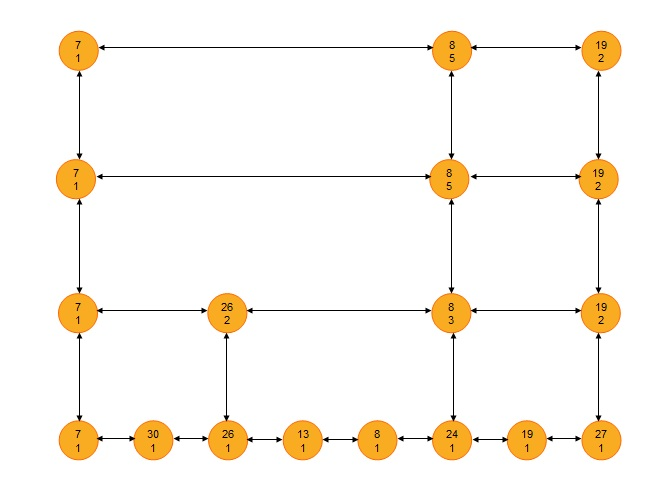
\includegraphics[width=4in]{images/AugmentedSkipList.jpg}
    \caption{An Augmented Skip List}
    \label{fig:AugmentedSkipList}
  \end{center}
\end {figure}


\subsection{Finding the $i$-th element}

To do this, we start with the element at the root, and then we follow
the following steps:
\begin{enumerate}
\item Take the right pointer, if you do not overshoot the index.
\item Otherwise, take the down pointer.
\end{enumerate}

We argue that this is the same as finding a path from a leaf node to
the root node, which is of length $O(\lg{n})$ w.h.p. Therefore, the
running time of finding the $i$-th element in the augmented Skip List
is $O(\lg{n})$ w.h.p.

\begin{figure}[h!]
  \begin{center}
    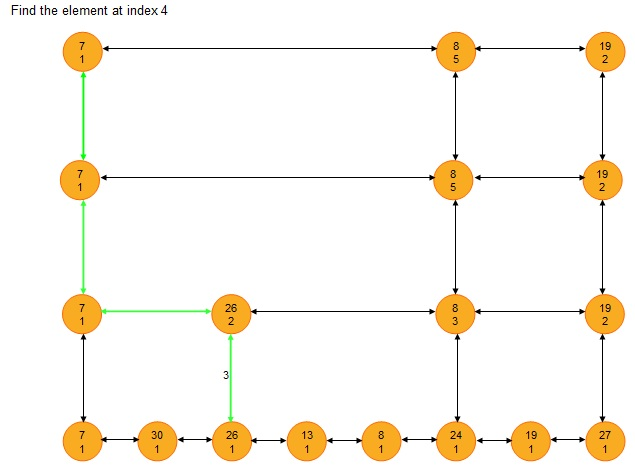
\includegraphics[width=4in]{images/Indexable.jpg}
    \caption{Indexing into an Augmented Skip List}
    \label{fig:Indexable}
  \end{center}
\end {figure}



\clearpage

\section{Range Minimum Query}

A `Range Minimum Query' (RMQ) is a query of type $Min(i,j)$, which
returns the minimum element between the indices $i$ and $j$.

In this section, we show how we can do Range Minimum Query using Skip
Lists, with $O(\lg{n})$ time for all $Min(i,j)$, $Insert(elem,
index)$, and $Delete(index)$ operations with high probability.

We further augment the Skip List, such that each node, at each level,
also stores the minimum value of \emph{leaf nodes} contained between
itself (included) and its predecessor on the same level (not
included).

\subsection{$Min(i,j)$}

In the augmented Skip List, we can break any given range, $[i,j]$ into
$k$ ranges, $(i-1,x_0]$, $(x_0, x_1]$, ..., $(x_{k-1}, j]$, where $k$
      is $O(\lg{n})$ w.h.p.  Each of these ranges is a single
      horizontal line on some level in the Skip List, and the value
      can be read off from the right hand side node on each of these
      horizontal lines.

To find such ranges, we start from the root, and find our way down, as
shown in Figure ~\ref{fig:MinInRange}.

\begin{figure}[h!]
  \begin{center}
    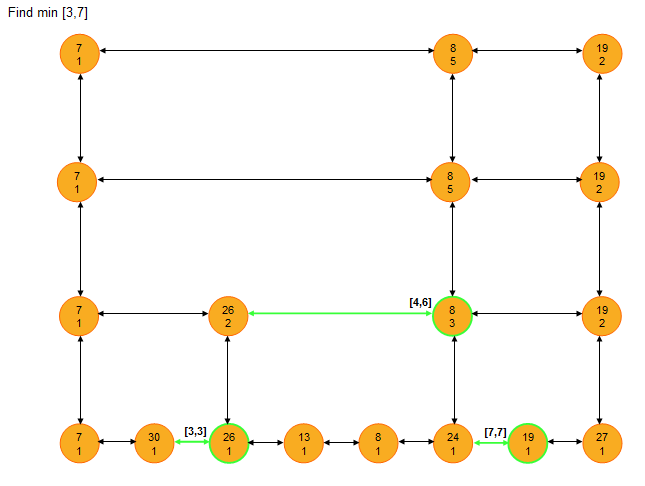
\includegraphics[width=4in]{images/MinInRange.jpg}
    \caption{Finding the Minimum in the range $[3,7]$ in an Augmented Skip List}
    \label{fig:MinInRange}
  \end{center}
\end {figure}

\clearpage

\subsection{$Insert(elem, index)$}

To insert an element, we follow the standard routine. However, we
would need to recompute the count and minimum value attributes for
each of the left and right neighbors of the node, as the node
propagates upwards. This can be visualized again as a set of
horizontal lines on the path connecting the predecessor (or successor)
of the inserted node at a given level to the inserted node at the
lowest level.

This is done as shown in Figure ~\ref{fig:Insert}, where the purple lines denote
the path from the predecessor of the inserted node at every level to
the inserted node at the lowest level.  Similarly, the blue lines
perform the same function for the successor nodes at each level.


\begin{figure}[h!]
  \begin{center}
    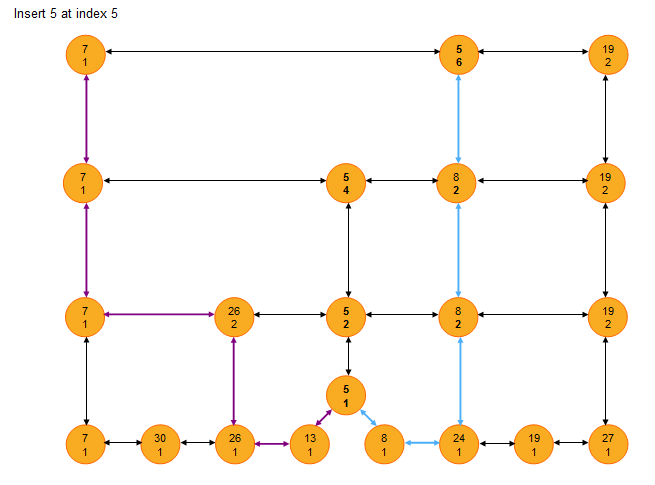
\includegraphics[width=4in]{images/Insert.jpg}
    \caption{Inserting the value 5 at index 5 in an Augmented Skip List}
    \label{fig:Insert}
  \end{center}
\end {figure}



\clearpage

\section{Order Maintenance}

To perform Order Maintenance, we insert an element after a given
element. This costs $O(\lg{n})$ w.h.p.

To find if an element $x$ precedes, $y$, we only need to check if
$rank(x) \leq rank(y)$.  We can find the rank of an element in a way
similar to indexing and this would cost us $O(\lg{n})$ w.h.p.


\begin{figure}[h!]
  \begin{center}
    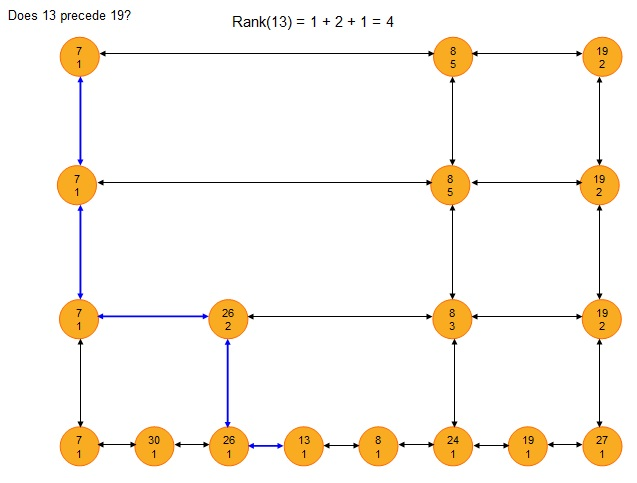
\includegraphics[width=4in]{images/OrderMaintenance1.jpg}
    \caption{Finding the rank of element 13 in an Augmented Skip List}
    \label{fig:OrderMaintenance1}
  \end{center}
\end {figure}



\begin{figure}[h!]
  \begin{center}
    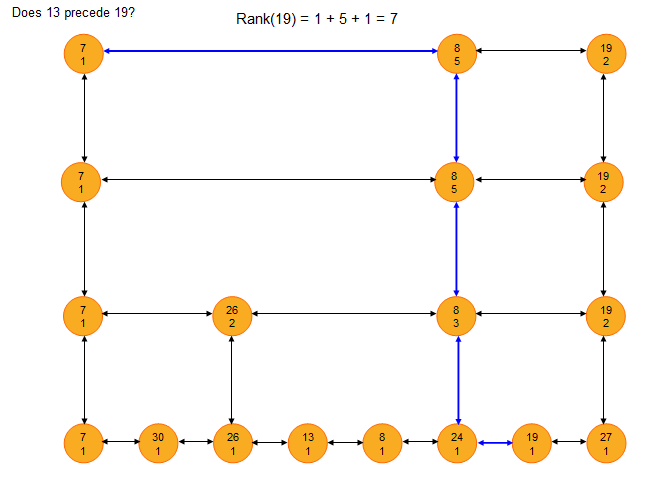
\includegraphics[width=4in]{images/OrderMaintenance2.jpg}
    \caption{Finding the rank of element 19 in an Augmented Skip List}
    \label{fig:OrderMaintenance2}
  \end{center}
\end {figure}

\clearpage

\begin{thebibliography}{}

\bibitem{} 
Skip lists: a probabilistic alternative to balanced trees,
William Pugh,
1990.

\bibitem{}
A Skip List Cookbook,
William Pugh,
1990.

\bibitem{} 
Prof. Eric Demaine's Order Maintenance notes,
Spring 2012 \\
\url{http://courses.csail.mit.edu/6.851/spring12/lectures/L08.pdf}.

\end{thebibliography}{}

\end{document}
